\documentclass[]{scrartcl}
\usepackage{graphicx}
\usepackage{color}
\usepackage{german}
\usepackage{hyperref}
%\pagestyle{headings}

\begin{document}

\title{
	\includegraphics*[width=0.75\textwidth]{images/hu_logo.png}\\
	\vspace{24pt}
	Die G"odelschen Unvollst"andigkeitss"atze}
\subtitle{Vorlesung WS 16/17\\
          Prof. Dr. Karl-Georg Niebergall\\
          Philosophisches Institut I \\ 
          Humboldt Universit"at zu Berlin}
\author{Lennard Wolf\\
        \href{mailto:lennard.wolf@student.hu-berlin.de}{lennard.wolf@student.hu-berlin.de}}
\maketitle
\begin{abstract}

Die G"odelschen Unvollst"andigkeitss"atze – „Die Peano-Arithmetik ist unvollst"andig“ (das 1. G. Theorem) und „Die Konsistenz der Peano-Arithmetik ist in dieser nicht beweisbar“ (das 2. G. Theorem) – und Verallgemeinerungen von diesen geh"oren zu den grundlegenden und wichtigsten Resultaten der Logik. 

Nach einer kurzen Einf"uhrung in die Philosophie der Mathematik des fr"uhen 20 Jhdt. zeige ich ausf"uhrlich das 1. G. Theorem (in der o.g. Form). Dieser Beweis sowie die Behandlung von Verallgemeinerungen stehen im Zentrum dieser Vorlesung. Der Beweis wird direkt gef"uhrt, ohne 
z.B. die Benutzung von rekursionstheoretischen Mitteln. Eine wichtige Rolle werden dabei vielmehr Untersuchungen der Komplexit"at von gewissen arithmetischen Formeln spielen. 

Zum Abschluss soll auf Beweisbarkeitslogik und, wenn auch nicht im Detail, auf das 2. G. Theorem eingegangen werden.

\end{abstract}
\newpage

\tableofcontents
\listoffigures
\newpage


\section{Vorbemerkungen\\(21.10.16)}

\subsection{G"odels Beweise}
\subsubsection{Hintergrund}

\begin{itemize}
  \item Wienerkreis: Dem Karnapp erkl"art (1930) und 1931, 1936 wesentliche Verfeinerung
  \item Gottlob Frege: Quantoren
  \item Principia Mathematica von Russel und Whitehead wurde von G"odel als unvollst"andig bewiesen (\emph{"Uber formal unentscheidbare S"atze der Principia Mathematica und verwandter Systeme I})
  \item Stellt Variante des Formalismus 
  \item Was ist Unvollst"andigkeitsbeweis?\\ $\rightarrow$ Satz $\phi$ ist unentscheidbar wenn nur $\phi$ oder $\neg~\phi$ beweisbar ist
\end{itemize}

\subsubsection{(G1.i)}

\textbf{Keine rekursiv aufz"ahlbare Erweiterung von $PA$ ist vollst"andig.}
\newline

Wenn $T$ eine konsistente r.a. Erweiterung von $PA$ in $L(PA)$ ist, dann gibt es einen Satz $\psi$ in $L(PA)$, so dass $T$ $\not \vdash$ $\psi$ und $T$ $\not \vdash$ $\neg~\psi$

\begin{itemize}
  \item Peano Arithmetik ($PA$) und $L(PA)$ ist die Sprache "uber $PA$
  \item \emph{r.a.}: rekursiv aufz"ahlbar
  \item ben"otigstes Wissen: Modelle $<M, J>$ und $<M, R1M, R2M, f1M, a1m, a2m, a3m>$
\end{itemize}

\subsubsection{(G1.ii)}
\textbf{Keine rekursiv aufz"ahlbare Erweiterung von $PA$ beweist ihre eigene Konsistenz.}
\newline

Wenn $T$ eine konsistente r.a. Erweiterung von $PA$ in $L(PA)$ ist, dann gibt es einen Satz $\psi$ in $L(PA)$, so dass $T$ $\not \vdash$ $\psi$ und $\psi$ wahr (im Standardmodel $N$) ist

\begin{itemize}
  \item Hintergrund: Hilbert's Programm
  \item $\rightarrow$ Mengenlehre, Russel'sche Antinomie ($\{ X | X \notin X \}$)
  \item $\rightarrow$ Formalismus und Finitismus
  \item $\rightarrow$ G"odelsche Theoreme
\end{itemize}

Wann ist Theorie $T$ widerspruchsfrei? $\rightarrow$ wenn $T \vdash (0 = 1)$


\subsection{Grundlegung der Mathematik}

3 Positionen (in den 20ern)

\begin{itemize}
  \item Logizismus (Frege, Russel/Whitehead, Wiener Kreis) $\rightarrow$ aufgegeben
  \item Formalismus (Hilbert) $\rightarrow$ G"odel, Semantik
  \item Intuitionismus (Brouwer, Heyting) $\rightarrow$ Minderheit
\end{itemize}

Positionen heute

\begin{itemize}
  \item Intuitionismus $\rightarrow$ Minderheit
  \item Platonismus  $\rightarrow$ indispensability
  \item Nominalismus $\rightarrow$ zu schwach
  \item Strukturalismus $\rightarrow$ ???????
  
\end{itemize}

Klassisch in der Ontologie: Platonismus, Normalismus, Konzeptualismus
\newline

1930 K"onigsberg Kongress zur Grundlegung der Mathematik (in Zeitschrift \emph{Erkenntnis} ver"offentlicht)

transfinite Scheinaussage


\section{Motivation \& Peano Arithmetik\\(28.10.16)}

`Der Satz an der Tafel ist falsch'
Bezeichner: `Der Satz an der Tafel'
Bezeichner ist wahr
$\rightarrow$ auch lowlevel gibt es dieses Paradox

Dieser Satz ist falsch. --Lünersatz
Dieser Satz ist nicht wahr. --verstärkter Lügnersatz

Dieser Satz ist nicht beweisbar. -- goedel satz
Dieser Satz ist nicht in T herleitbar. --T=eine Theorie
Dieser Satz ist nicht herleitbar. --in allen Theorien
TODO antinomie

beweisbar hier rein logisch beweisbar
herleitbar hier beweisbarkeit in logischer theorie

PA hat das Ziel der maximalkonsistenz
Dieser Satz ist nicht PA-herleitbar. --wenn der Satz nicht deutsch sondern in L(PA) ist, wären wir fertig
\newline
\textbf{Unser System:}

$\langle~\neg$, $\rightarrow$, $\forall , v_{0},v_{1}, ... , v_{n}, \bar{0}$, $\bar{S}$, $\bar{+}$, $\bar{*}$, $\bar{<}$, $\bar{=}$, $\bar{(}$, $\bar{)}~\rangle$
\newline
\textbf{Metasprache:}

doppelt gestrichene nicht,impication, all-quantor, x,x0...,z,y..., 0,S,+,*,<,element zeichen
\newline
\textbf{Axiome:}
Vv0: nicht Sv0 = 0
Vv0,v1: Sv0=Sv1->v0=v1
Vv0: v0+0=v0
Vv0v1: v0+Sv1 = S(v0+v1)
Vv0: v0*0=0
Vv0,v1: v0*Sv1 = v0*v1 + v0
induktionsschema: sei q eine L(PA) formel dann ist q(0)andVv0:(q(v0)->q(Sv0))->Vv0:q(v0) eine instanz des induktionsschemas
induktionsschema sind undendlich viele axiome... ;( but geht not otherwise
schema != regel // schema ist eine menge von sätzen 
PA := {q| q Formel aus L(PA) und AxPA |- q} --q ist formel und aus axiomen herleitbar

coole Leute: 
Moore, Goldfarb, Quine, Kalmar, Hilbert

wichtiger crap:
gebrauch-erwähnungsunterscheidung

\section{Vorbemerkungen II\\(04.11.16)}

\begin{itemize}
  \item `$\bar{0}$' ist ein Numeral.
  \item `$\bar{S}\bar{0}$' ist ein Numeral. (ein Konkatenat) Zeichen finden! kleiner schweif dazwischen
  \item `$\bar{S}\bar{0}$' $=$ `$\bar{S}$' ?? `$\bar{0}$'
  \item $0$ ist eine \emph{Instanz} einer nat"urlichen Zahl.
  \item 
\end{itemize}




PA ist vollst"andig f"ur quantorenfreie S"atze.

%\begin{figure}[h]
%	\centering
%	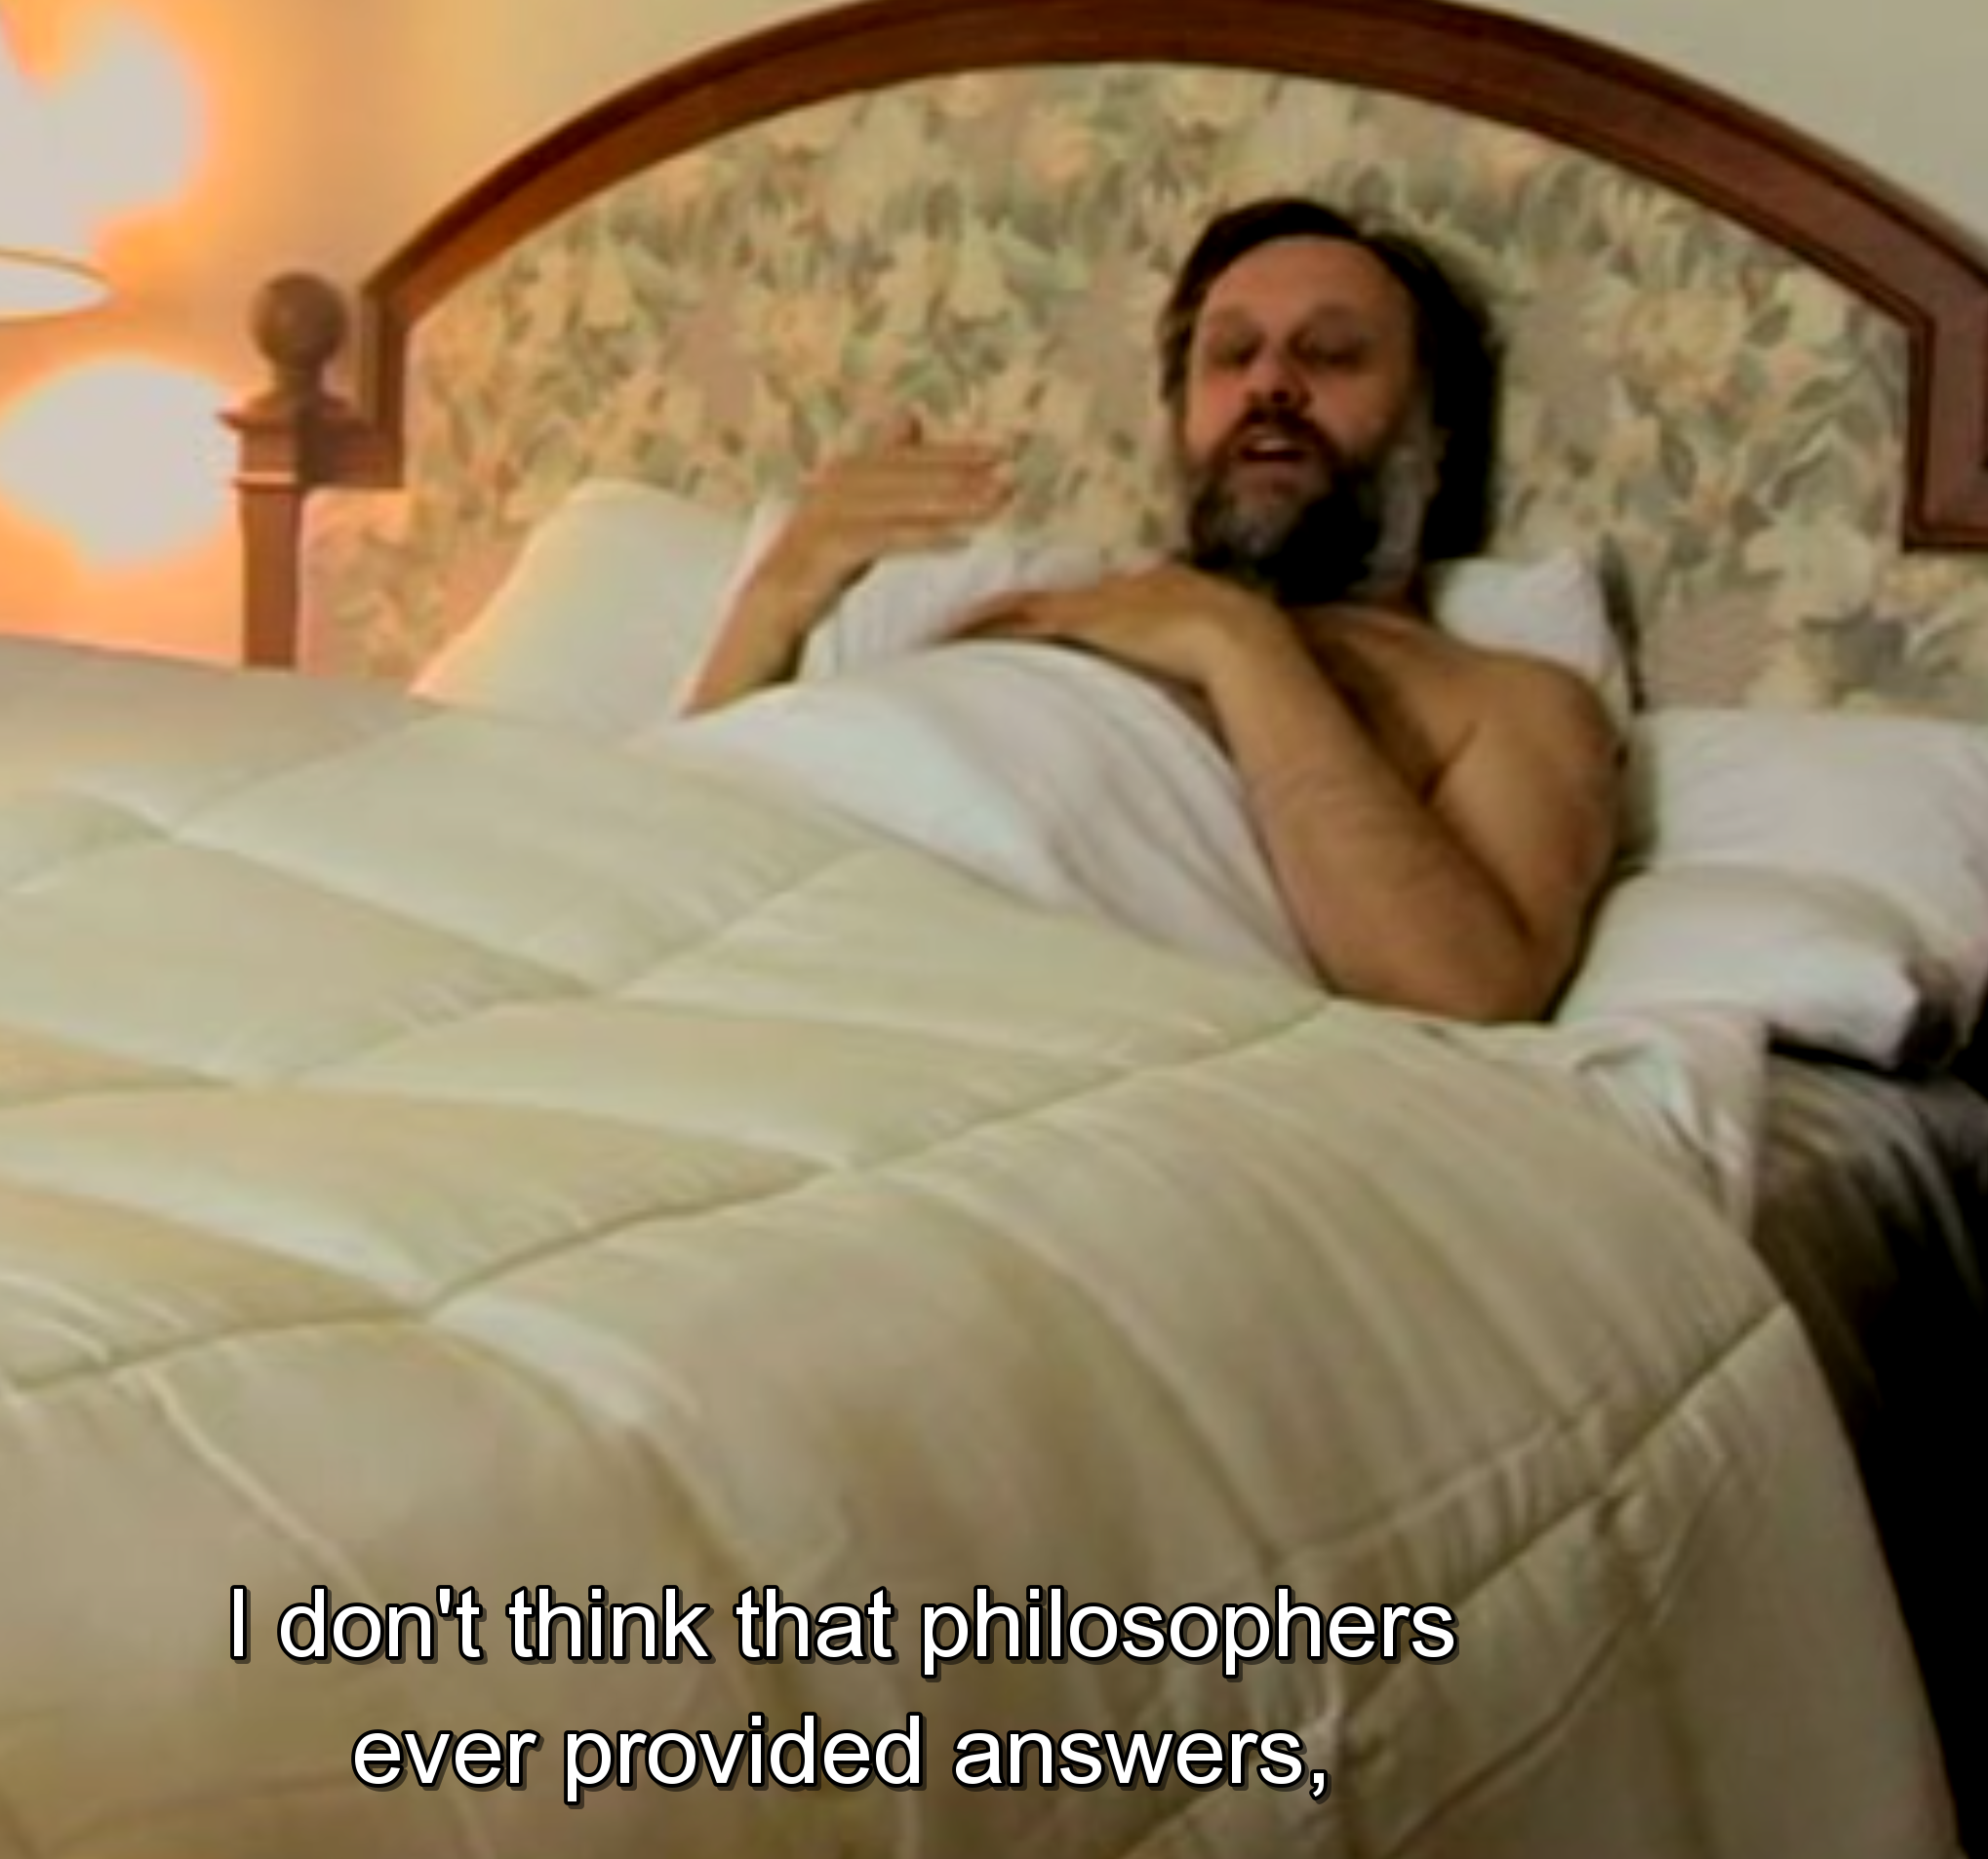
\includegraphics[width=0.5\textwidth]{images/template.png}
%	\caption{Template Bild}
%	\label{fig:template}
%\end{figure}



\newpage
\section{"Uber den Professor}
Prof. Mustermann ist..


\end{document}
